\section{Sustainable Energy Sources}

\begin{multicols}{2}


\section*{Water Energy}


\subsection{Water Wheel}

\begin{center}
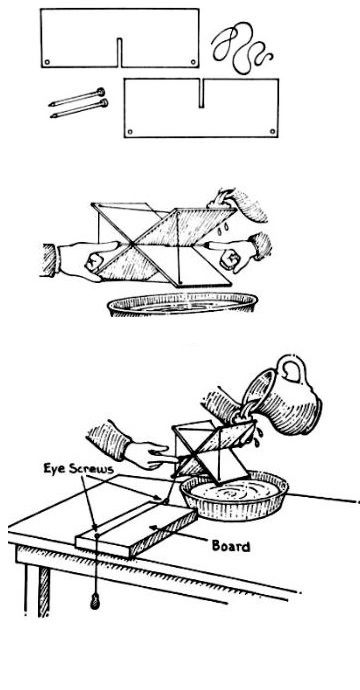
\includegraphics[width=0.5\textwidth]{./img/water-wheel.jpg}
\end{center}

\begin{description*}
%\item[Subtopic:]{}
\item[Materials:]{Stiff cardboard, scissors, nails, string, water, basin}
\item[Setup:]{Construct the water wheel as shown.}
\item[Procedure:]{Tie a small weight (e.g. paperclip, nail) to the string so that it rests on the floor. Pour water over the water wheel to turn it and lift the weight. }
%\item[Hazards:]{}
%\item[Questions:]{}
%\item[Observations:]{}
\item[Theory:]{Water stores potential energy in the forms of rivers and waterfalls and when placed in an elevated storage tank. The kinetic energy of falling water can be used to do work on an object and generate electricity.}
\item[Applications:]{\nameref{sub:water-turbine} (p.~\pageref{sub:water-turbine}).}
%\item[Notes:]{}
\end{description*}

\columnbreak

%==================================================================================================%

\section*{Solar Energy}


\subsection{Energy from the Sun}

\begin{center}
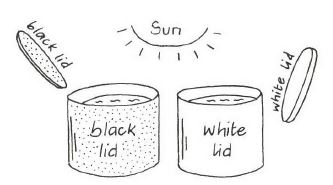
\includegraphics[width=0.4\textwidth]{./img/vso/solar-heat.jpg}
\end{center}

\begin{description*}
%\item[Subtopic:]{}
\item[Materials:]{2 tins or cans, black paint/shoe polish, aluminum foil}
\item[Setup:]{Paint one tin black and cover the other with aluminum foil.}
\item[Procedure:]{Place both tins out in the sun. Leave for 15 minutes and then feel them.}
%\item[Hazards:]{}
%\item[Questions:]{}
\item[Observations:]{The black tin is warmer.}
\item[Theory:]{The sun's energy gets absorbed by objects on earth. Dark surfaces absorb more energy than bright and reflective surfaces.}
%\item[Applications:]{}
%\item[Notes:]{}
\end{description*}

%==================================================================================================%

\section*{Wind Energy}


\subsection{Windmills}

\begin{center}
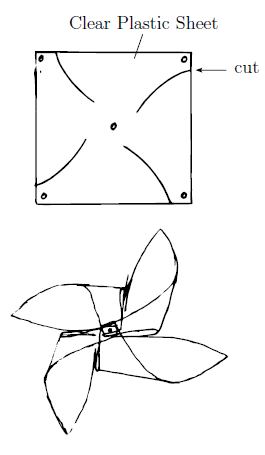
\includegraphics[width=0.49\textwidth]{./img/windmill.png}
\end{center}

\begin{description*}
%\item[Subtopic:]{}
\item[Materials:]{Paper/thin cardstock, scissors, pen, glue, paper fastener/thumb tack, straw or stick, colored pencils (optional)}
%\item[Setup:]{}
\item[Procedure:]{Copy the illustration onto a sheet of paper or thin cardstock. Cut along the lines and make holes with a pen. Bend the four corners together into the center and glue them in place. Push the fastener through the center into a straw or stick.}
%\item[Hazards:]{}
%\item[Questions:]{}
%\item[Observations:]{}
\item[Theory:]{Wind provides kinetic energy which can be harnessed with a device such as a windmill and used to generate electricity if connected to a turbine.}
\item[Applications:]{\nameref{sub:wind-turbine} (p.~\pageref{sub:wind-turbine}).}
%\item[Notes:]{}
\end{description*}

%==================================================================================================%



\end{multicols}

\pagebreak